\subsection{Grundfunktionen des Dojos}
Die Funktionalität wurde von der Auftraggeberin Jana Kalbermatten ausgearbeitet. Nachfolgend wird die alltägliche Nutzung des Dojos aus Sicht des Benutzers sowie des Museumsmitarbeiters erklärt.
\subsubsection{Aufladen des Akkus}
Zum Laden wird der Dojo an eine Ladevorrichtung oder eine Ladestation angebracht. Dabei wird ein Mikro-USB Kabel an den Dojo angeschlossen. Alternativ kann eine Ladestation mit mehreren Steckplätzen realisiert werden, an welcher mehrere Dojos gleichzeitig geladen werden können.
\begin{figure}[htb]
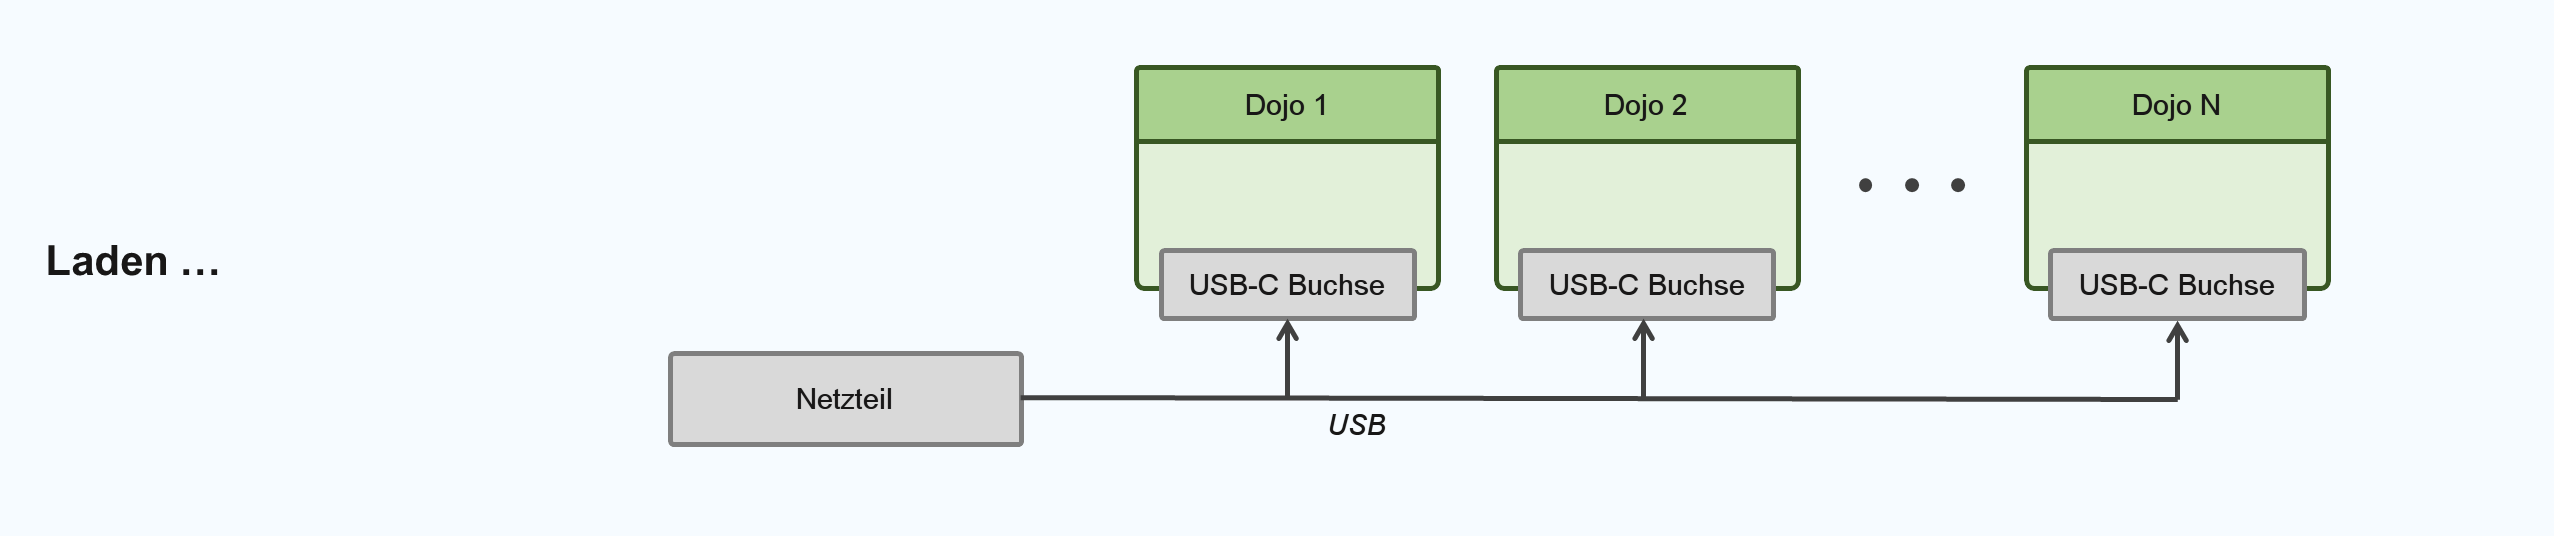
\includegraphics[width=\textwidth]{Zustand_Laden.png}
\caption{Zustand beim Laden} % picture caption
\label{fig:image2}
\end{figure}
\subsubsection{Konfigurieren einer Ausstellung}
Vor der Eröffnung einer neuen Ausstellungen müssen die Audiodateien auf den Dojo geladen werden. Dies geschieht mit dem Verbinden des Dojos auf einen Computer mittels Mikro-USB Kabel. Die SD-Karte auf dem Dojo wird dadurch im Dateiverzeichnis des Computers sichtbar. Durch unsere Java-Applikation kann eine Ausstellung mit den verschiedenen Audiodateien zusammengestellt und die entsprechenden Beacon IDs sowie der dazugehörigen Sprache gesetzt werden. Die Software überträgt anschliessend die Dateien mit der korrekten Codierung.
\begin{figure}[htb]
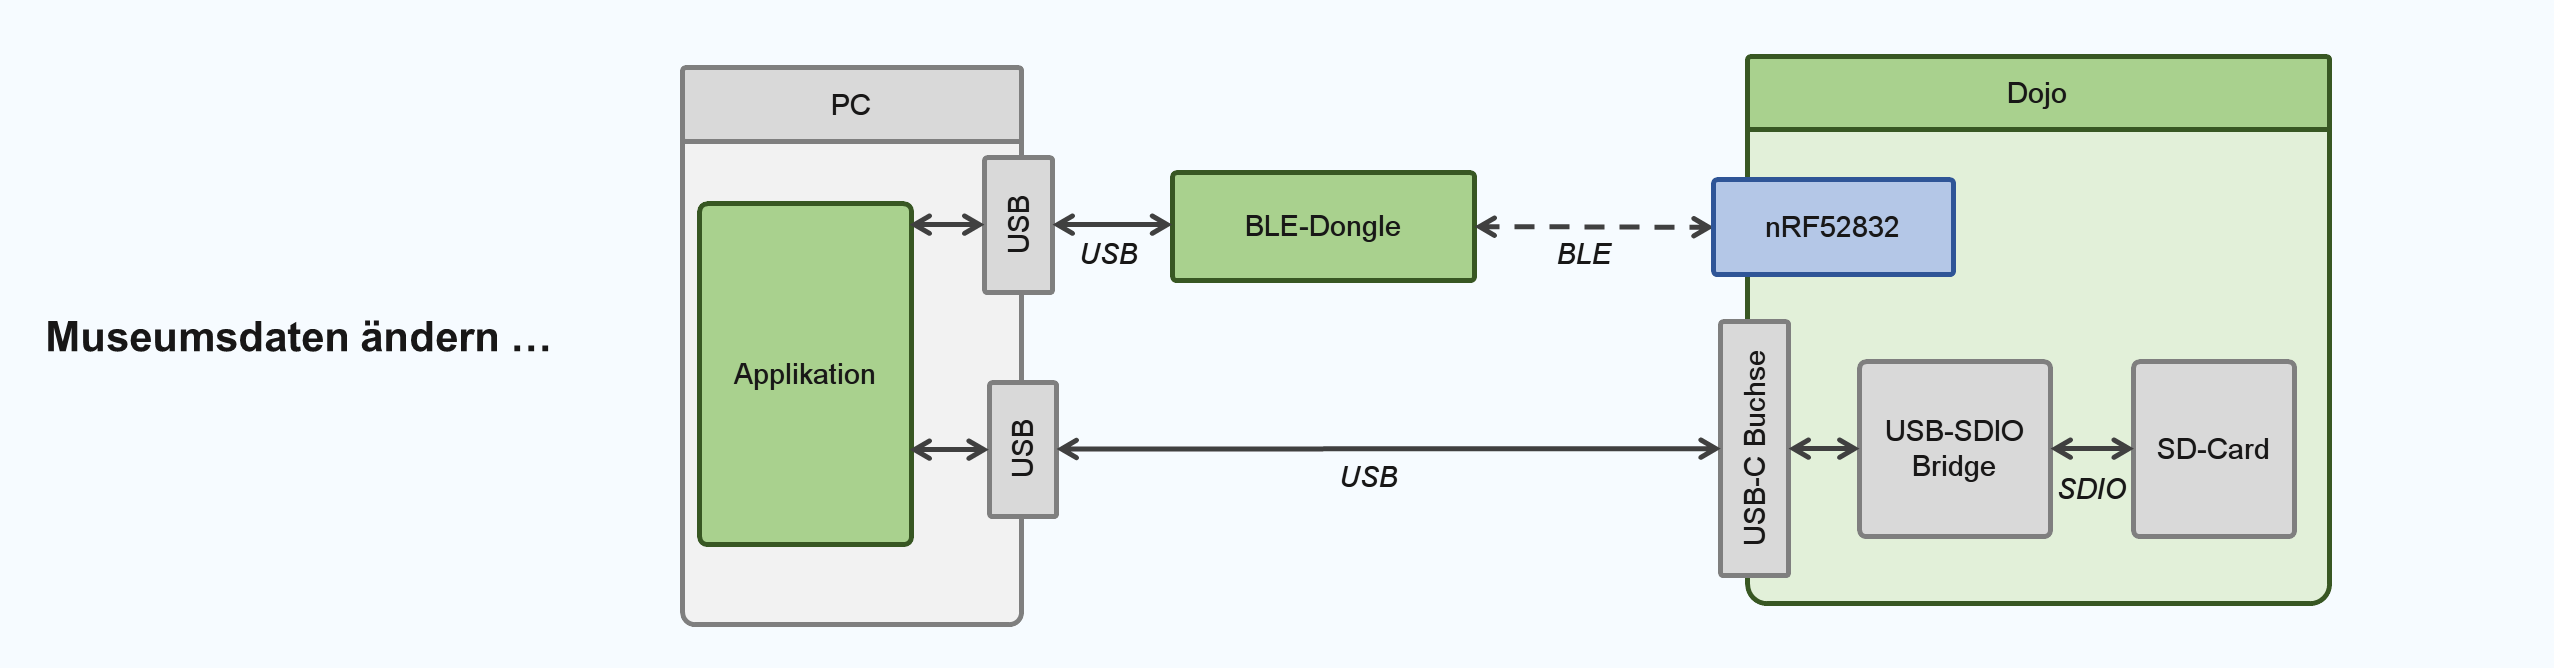
\includegraphics[width=\textwidth]{Zustand_Programmieren.png}
\caption{Zustand beim Programmieren} % picture caption
\label{fig:image3}
\end{figure}
\subsubsection{Konfigurieren eines Dojos}
Die Zutritts- und die Sprachinformationen werden beim Start des Museumsbesuches durch den Rezeptionisten auf den Dojo geladen. Diese Übertragung funktioniert drahtlos über Bluetooth. Es ist auch möglich, während des Besuches neue Berechtigungen zu erwerben und den Dojo entsprechend zu aktualisieren.
\begin{figure}[htb]
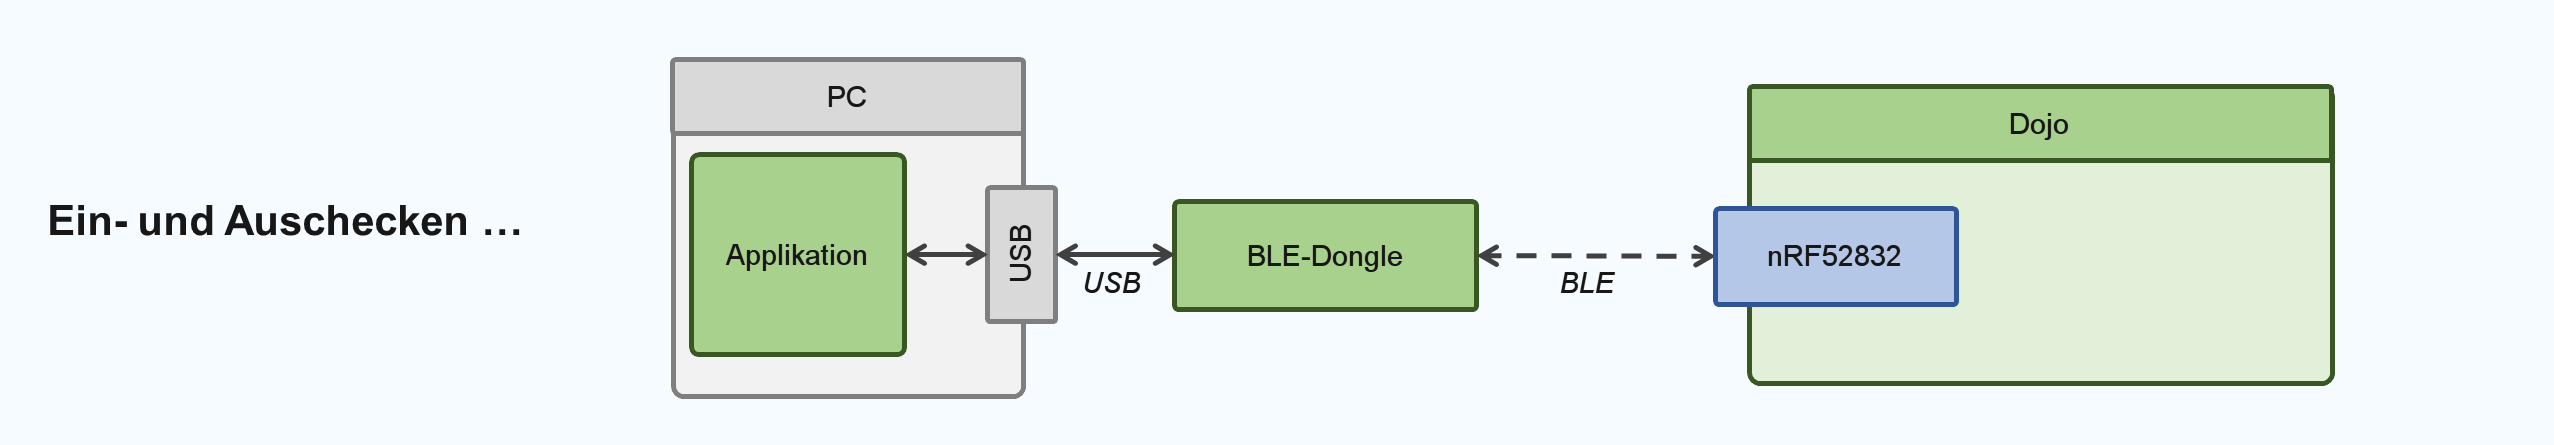
\includegraphics[width=\textwidth]{Zustand_Ein_Aus_Checken.png}
\caption{Zustand beim Ein- und Auschecken} % picture caption
\label{fig:image1}
\end{figure}
\subsubsection{Museumsrundgang mit dem Dojo}
Während des Rundgangs hat der Dojo zwei Funktionen. Die Hauptfunktion ist das Lokalisieren von Bluetooth Beacons und das Abspielen der dazugehörigen Informationen vor einem Objekt. Wenn der Besucher mit dem Dojo in die Nähe eines Objektes kommt, vibriert dieser kurz, um dem Besucher das Vorhandensein einer Audiodatei zu signalisieren. Drückt der Besucher die Play-Taste, so wird die Audiodatei abgespielt.Diese kann durch den Knochenschallgeber, welcher sich am oberen Ende des Dojos befindet, angehört werden....(line truncated)...
Eine weitere Funktion, die im Prototypen eingebaut wurde, ist die Zugangsberechtigung. Das Museum kann eine Ausstellung in verschiedene Bereiche unterteilen. Der Dojo dient als elektronisches Ticket für die einzelnen Bereiche. Ähnlich wie ein Badge muss er dafür nur an eine Konsole gehalten werden. Der Dojo stellt automatisch eine Verbindung mit der Station her und tauscht seine Berechtigungen aus. Wurde die Berechtigung bei der Rezeption erteilt, so wird der Durchgang geöffnet. Diese Funktion kann beispielsweise beim Haupteingang nach der Rezeption mit einem Drehkreuz verwendet werden oder bei mehreren Ausstellungen in verschiedenen Räumen.
\begin{figure}[htb]
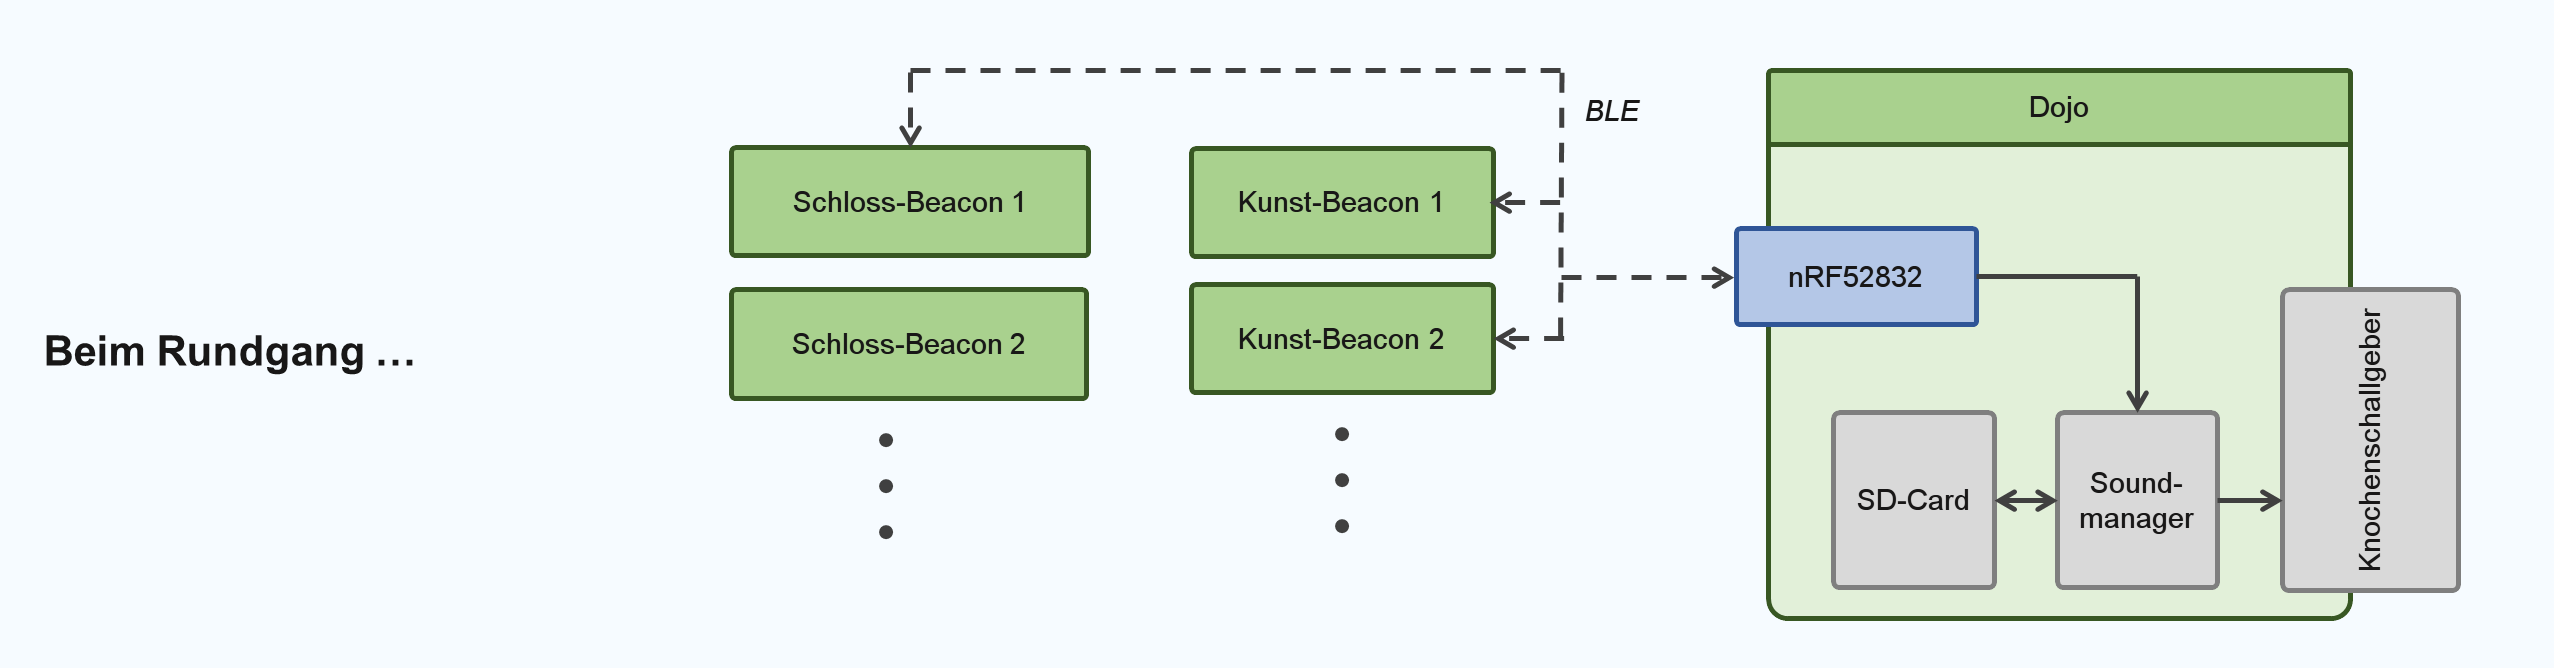
\includegraphics[width=\textwidth]{Zustand_Rundgang.png}
\caption{Zustand beim Rundgang} % picture caption
\label{fig:image4}
\end{figure}











\clearpage
\subsection{Mechanischer Aufbau des Dojos}
Das Design des Dojos aus Abbildung \ref{fig:DojoBild} wurde für die Bachelorarbeit von Jana Kalbermatten erarbeitet und dient als Vorlage für das Gerät. Der Dojo ist mit $245mm$ ziemlich lang, besitzt jedoch mit einem Aussendurchmesser von nur $19.5mm$ einen kleinen Querschnitt. Dieses Gehäuse setzt eine detaillierte Planung der elektronischen Bauteile voraus sowie ein kompaktes Design der elektronischen Schaltung.



\begin{figure}[h]
	\centering
	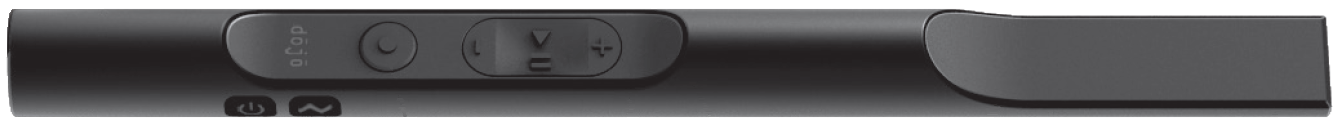
\includegraphics[width=\textwidth]{graphics/DojoBild.png}
	\caption{Aussenansicht des Dojos}
	\label{fig:DojoBild}
\end{figure}

Durch den begrenzten Durchmesser und der begrenzten Schiebeöffnung auf der Rückseite des Dojos kommen keine Akkumulatoren der Normgrösse $A$ sowie $AA$ infrage. Eingebaut wird daher ein Akkumulator der Grösse $AAA$. Um mit den Tastern und dem USB-Port nicht in Konflikt zu geraten, wird der Akkumulator in der Mitte des Dojos eingebaut siehe Abbildung \ref{fig:DojoQuerschnitt}. Dies hat ebenfalls den Vorteil, das man einen Print der Länge $120mm$ einbauen kann, welcher den USB Port, sowie alle Taster beinhaltet


\begin{figure}[h]
	\centering
	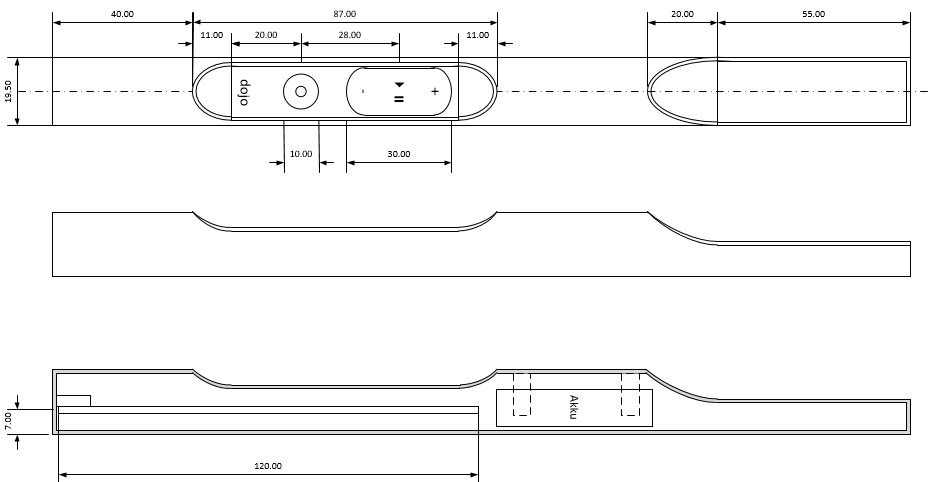
\includegraphics[width=\textwidth]{graphics/DojoQuerschnitt.png}
	\caption{Technische Zeichnung des Dojos}
	\label{fig:DojoQuerschnitt}
\end{figure}

\newpage

Der Akkumulator wird mit einer Batteriehalterung in das Gehäuse verbaut. Dabei bleibt, wie in der Abbildung \ref{fig:DojoAkkumulatorQuerschnitt} zu sehen, neben der Halterung genügend Platz für die Verbindungskabel, welche zum Knochenschallgeber am Ende des Dojos führen. Ebenfalls kann der Akkumulator durch den Schiebeöffner an der Rückseite des Dojos entfernt werden.


\begin{figure}[h]
	\centering
	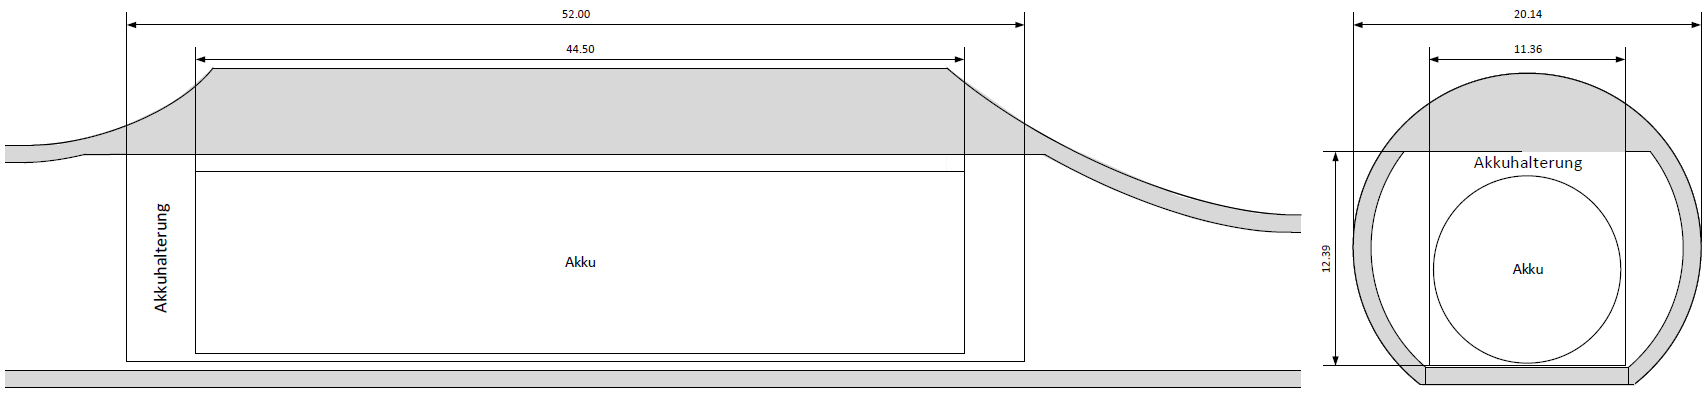
\includegraphics[width=\textwidth]{graphics/DojoAkkumulatorQuerschnitt.png}
	\caption{Positionierung des Akkumulators}
	\label{fig:DojoAkkumulatorQuerschnitt}
\end{figure}

Der Print nimmt mit einer Länge von $120mm$ und einer Breite von $17mm$ den grössten Teil des Gehäuses in Beanspruchung. Aufgrund der hohen Komplexität der elektronischen Schaltung handelt es sich um einen mehrlagigen Print. Am unteren Ende des Dojos befindet sich die Buchse der USB-Verbindung. Diese wird, wie in Abbildung \ref{fig:DojoPrintQuerschnitt} dargestellt, auf dem Print motiert. Die zweite Darstellung zeigt einen Querschnitt des Dojos bei den Tasten. Diese können auf dem Print befestigt und mechanisch mit den Tastern des Gehäuses verbunden werden. Am oberen Ende des Prints werden die Kontakte für die Batterie sowie den Knochenschallgeber angebracht.


\begin{figure}[h]
	\centering
	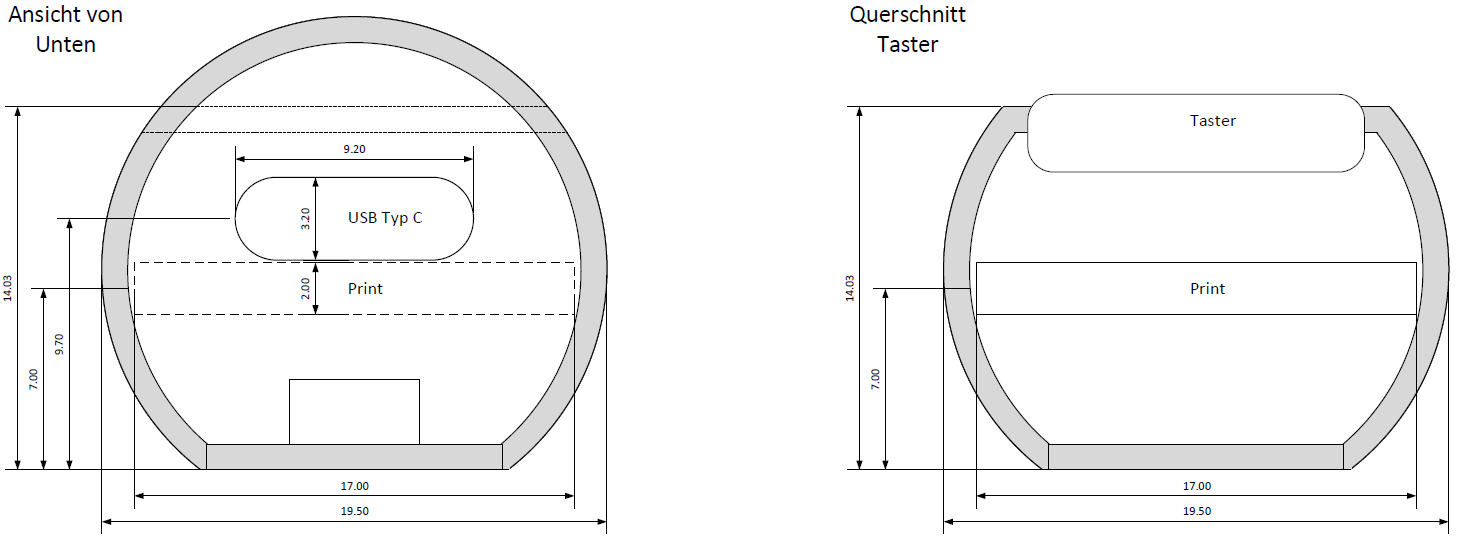
\includegraphics[width=\textwidth]{graphics/DojoPrintQuerschnitt.png}
	\caption{Positionierung des Prints}
	\label{fig:DojoPrintQuerschnitt}
\end{figure}


